\documentclass[a4paper,10pt]{report}
\usepackage[utf8]{inputenc}

%multiline comments
\usepackage{verbatim}

%derivatives, ...
\usepackage{physics}

%for images
\usepackage{pgf}
\usepackage{tikz}
\usetikzlibrary{shapes,snakes}
\usepackage{subfig}

%math symbols
\usepackage{amsmath}
\usepackage{amssymb}

%SI package
\usepackage{siunitx}

%line between paragraphs
\usepackage[parfill]{parskip}

\usepackage{geometry}
 \geometry{
 a4paper,
 total={160mm,227mm},
 left=30mm,
 right=30mm,
 top=30mm,
 }

%code listing
\usepackage{listings}

%opening
\title{Design of a machine learning model for the detection of young planets}
\author{Alessandro Ruzza}

\begin{document}

\maketitle

\addcontentsline{toc}{chapter}{Abstract}
\begin{abstract}
    Protoplanetary discs present substructures,
    such as axisymmetric regions of luminosity depletion (gaps),
    that can be explained by the presence of forming planets. 
    Features of these objects can be inferred from their
    observation and analysis. A remarkable example is the 
    estimation of the planetary mass from the gaps morphology.
    The approaches currently used, empirical formulae or numerical
    simulations, are both limited in precision or applicability.
    In this thesis we propose a machine learning approach:
    using a neural network to infer this information from 
    disk images with the requirement of the least amount
    of physical features not directly observable.
    Possible future developments of such models require 
    data for the train and test phases.
    We design and build a database for this purpose collecting 
    data obtained from numerical simulations and providing an 
    easy-to-use interface for the implementation of machine learning
    models using TensorFlow libraries.
\end{abstract}

\tableofcontents

\chapter{Introduction}


\chapter{Protoplanetary discs}
%Very brief introduction (1/2 sentences) about what a protoplanetary disc is,
%how they generate, where we can find them and why they are studied.

Protoplanetary discs emerge in the context of star formation. 
The process takes place in specific ``star forming'' regions filled with a mixture of gases, mainly hydrogen and helium enriched with some
heavier elements, called interstellar medium. The gravitational collapse of a denser zone gives birth to a star. Gradually the star
accrete its mass drawing, from its surroundings, gas and dust that organizes in an accretion disc whose shape is a consequence of angular momentum conservation.
At some point, after $\sim 10^5$ yr, most of the matter has accreted into the star,
the disc temperature and thermal emission are maintained by the star irradiation while gravitational collapse becomes negligible as a source of energy (passive disc). 
It is at this stage that the accretion disc get identified
as a protoplanetary disc due to its role as a planet formation cradle.
Their study allows the development and test of theoretical models regarding planets and their genesis.

In this chapter I am going to give an overview of the structure and observable features
of protoplanetary discs and of their relation with young embedded planets. The discussion will not be
exhaustive and neither detailed, the aim is to give
the reader a picture of these objects, and provide a basic understanding of the 
properties which I will be referring to in the next chapters.

\section{Structural properties}

\begin{figure}
    \begin{center}
    \raisebox{+0.2\height}{
        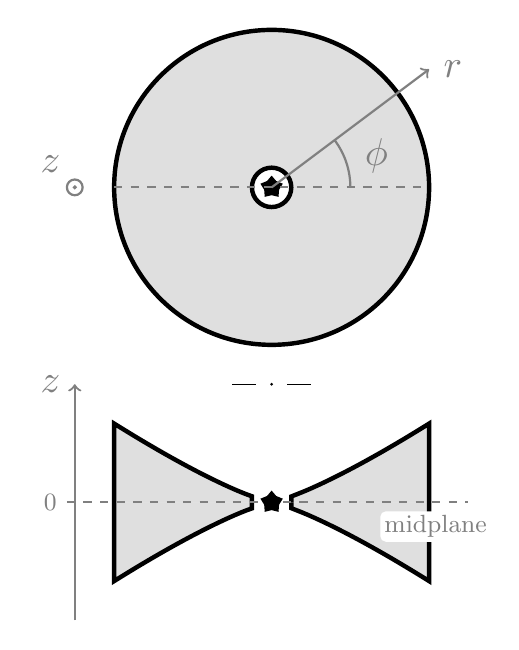
\begin{tikzpicture}
            \draw[ultra thick, color=black, domain=0.25:2, fill=gray, fill opacity=0.25] (0.25,0) -- plot (\x,{(\x*0.5)^(5/4)}) -- (2,0);
            \draw[ultra thick,color=black, domain=-2:-0.25, fill=gray, fill opacity=0.25] (-2,0) -- plot (\x,{(-\x*0.5)^(5/4)}) -- (-0.25, 0);
            \draw[ultra thick,color=black, domain=0.25:2, fill=gray, fill opacity=0.25] (0.25,0) -- plot (\x,{-(\x*0.5)^(5/4)}) -- (2,0);
            \draw[ultra thick,color=black, domain=-2:-0.25, fill=gray, fill opacity=0.25] (-2,0) -- plot (\x,{-(-\x*0.5)^(5/4)}) -- (-0.25,0);
            \draw[ultra thick,color=black] (2, 1) -- (2,-0.1);
            \draw[ultra thick,color=black] (2, -1) -- (2,-0.45);
            \draw[ultra thick,color=black] (-2, 1) -- (-2,-1);
            \draw[ thick,->, color=gray] (-2.5, -1.5) -- (-2.5, 1.5) node[left, scale=1.4] {$z$};
            \draw[ thick,color=gray, dashed] (-2.6, 0) node[left] {\small 0} -- (2.5, 0) node[below left, yshift=-1mm, xshift=3mm,  fill=white, rounded corners=2pt,inner sep=1.5pt] {\small midplane};
            \draw[ultra thick, fill=gray, fill opacity=0.25] (0,4) circle [radius=2cm];
            \draw[ultra thick, fill=white] (0,4) circle [radius=0.25cm];
            \node[star, fill=black, scale=0.6] at (0,4) {};
            \draw[ thick,color=gray] (-2.5,4) circle [radius=1mm] node[above left, scale=1.4] {$z$};
            \draw[ thick,color=gray, fill=gray] (-2.5,4) circle [radius=0.1mm];
            \draw[ thick,->, color=gray] (0,4) -- (2, 5.5) node[right, scale=1.4] {$r$};
            \draw[ thick,color=gray] (1,4) node[above right, scale=1.4] {$\phi$} arc (0:36.5:1cm);
            \draw[ thick,color=gray, dashed] (-2, 4) -- (2,4);
            \node[star, fill=black, scale=0.6] at (0,0) {};
            \draw[thin] (0, 1.5) circle [radius=0.1mm];
            \draw[thin] (0.2, 1.5) -- (0.5, 1.5);
            \draw[thin] (-0.2, 1.5) -- (-0.5, 1.5);
            %\draw[thin] (3, 1.5) circle [radius=0.1mm];
            %\draw[thin] (3, 1.3) -- (3, 1);
            %\draw[thin] (3, 1.7) -- (3, 2);
        \end{tikzpicture}}
        %\quadd
    %% Creator: Matplotlib, PGF backend
%%
%% To include the figure in your LaTeX document, write
%%   \input{<filename>.pgf}
%%
%% Make sure the required packages are loaded in your preamble
%%   \usepackage{pgf}
%%
%% Figures using additional raster images can only be included by \input if
%% they are in the same directory as the main LaTeX file. For loading figures
%% from other directories you can use the `import` package
%%   \usepackage{import}
%%
%% and then include the figures with
%%   \import{<path to file>}{<filename>.pgf}
%%
%% Matplotlib used the following preamble
%%
\begingroup%
\makeatletter%
\begin{pgfpicture}%
\pgfpathrectangle{\pgfpointorigin}{\pgfqpoint{3.380901in}{3.900000in}}%
\pgfusepath{use as bounding box, clip}%
\begin{pgfscope}%
\pgfsetbuttcap%
\pgfsetmiterjoin%
\pgfsetlinewidth{0.000000pt}%
\definecolor{currentstroke}{rgb}{1.000000,1.000000,1.000000}%
\pgfsetstrokecolor{currentstroke}%
\pgfsetstrokeopacity{0.000000}%
\pgfsetdash{}{0pt}%
\pgfpathmoveto{\pgfqpoint{0.000000in}{0.000000in}}%
\pgfpathlineto{\pgfqpoint{3.380901in}{0.000000in}}%
\pgfpathlineto{\pgfqpoint{3.380901in}{3.900000in}}%
\pgfpathlineto{\pgfqpoint{0.000000in}{3.900000in}}%
\pgfpathclose%
\pgfusepath{}%
\end{pgfscope}%
\begin{pgfscope}%
\pgfsetbuttcap%
\pgfsetmiterjoin%
\definecolor{currentfill}{rgb}{1.000000,1.000000,1.000000}%
\pgfsetfillcolor{currentfill}%
\pgfsetlinewidth{0.000000pt}%
\definecolor{currentstroke}{rgb}{0.000000,0.000000,0.000000}%
\pgfsetstrokecolor{currentstroke}%
\pgfsetstrokeopacity{0.000000}%
\pgfsetdash{}{0pt}%
\pgfpathmoveto{\pgfqpoint{0.746606in}{0.515123in}}%
\pgfpathlineto{\pgfqpoint{2.364932in}{0.515123in}}%
\pgfpathlineto{\pgfqpoint{2.364932in}{3.751775in}}%
\pgfpathlineto{\pgfqpoint{0.746606in}{3.751775in}}%
\pgfpathclose%
\pgfusepath{fill}%
\end{pgfscope}%
\begin{pgfscope}%
\pgfpathrectangle{\pgfqpoint{0.746606in}{0.515123in}}{\pgfqpoint{1.618326in}{3.236651in}}%
\pgfusepath{clip}%
\pgfsys@transformshift{0.746606in}{0.515123in}%
\pgftext[left,bottom]{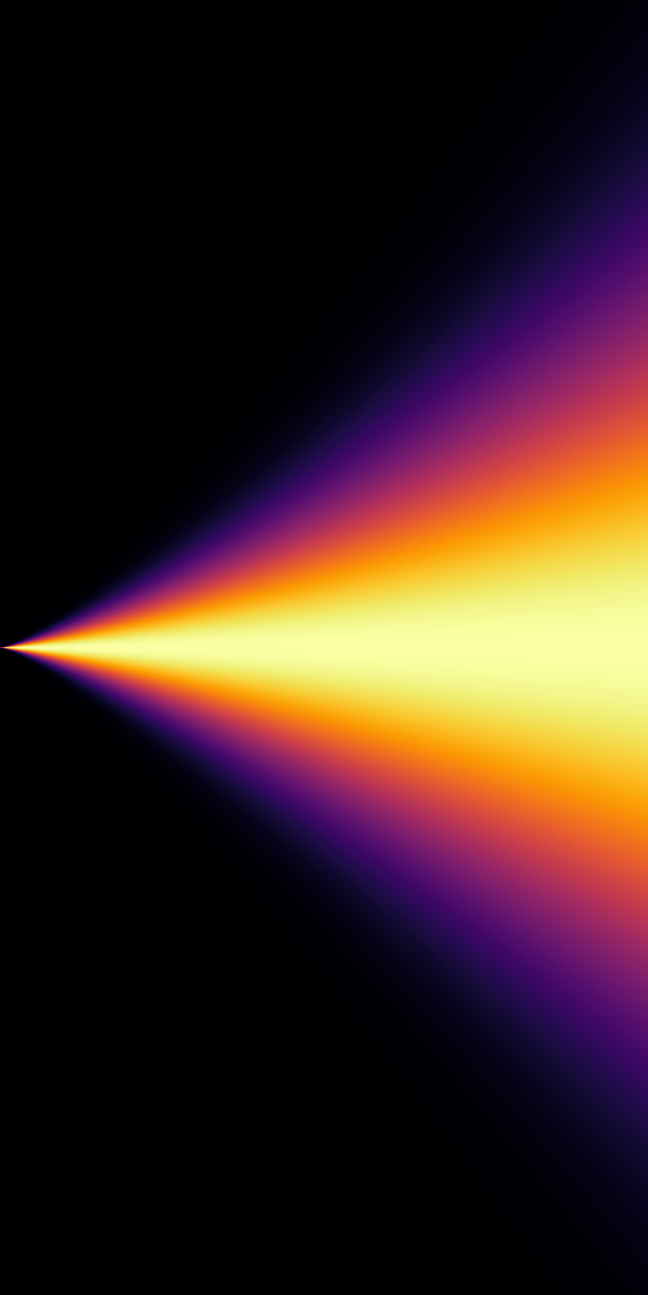
\includegraphics[interpolate=true,width=1.620000in,height=3.237500in]{images/profile-img0.png}}%
\end{pgfscope}%
\begin{pgfscope}%
\pgfsetbuttcap%
\pgfsetroundjoin%
\definecolor{currentfill}{rgb}{0.000000,0.000000,0.000000}%
\pgfsetfillcolor{currentfill}%
\pgfsetlinewidth{0.803000pt}%
\definecolor{currentstroke}{rgb}{0.000000,0.000000,0.000000}%
\pgfsetstrokecolor{currentstroke}%
\pgfsetdash{}{0pt}%
\pgfsys@defobject{currentmarker}{\pgfqpoint{0.000000in}{-0.048611in}}{\pgfqpoint{0.000000in}{0.000000in}}{%
\pgfpathmoveto{\pgfqpoint{0.000000in}{0.000000in}}%
\pgfpathlineto{\pgfqpoint{0.000000in}{-0.048611in}}%
\pgfusepath{stroke,fill}%
}%
\begin{pgfscope}%
\pgfsys@transformshift{0.746606in}{0.515123in}%
\pgfsys@useobject{currentmarker}{}%
\end{pgfscope}%
\end{pgfscope}%
\begin{pgfscope}%
\definecolor{textcolor}{rgb}{0.000000,0.000000,0.000000}%
\pgfsetstrokecolor{textcolor}%
\pgfsetfillcolor{textcolor}%
\pgftext[x=0.746606in,y=0.417901in,,top]{\color{textcolor}\rmfamily\fontsize{10.000000}{12.000000}\selectfont \(\displaystyle {0.0}\)}%
\end{pgfscope}%
\begin{pgfscope}%
\pgfsetbuttcap%
\pgfsetroundjoin%
\definecolor{currentfill}{rgb}{0.000000,0.000000,0.000000}%
\pgfsetfillcolor{currentfill}%
\pgfsetlinewidth{0.803000pt}%
\definecolor{currentstroke}{rgb}{0.000000,0.000000,0.000000}%
\pgfsetstrokecolor{currentstroke}%
\pgfsetdash{}{0pt}%
\pgfsys@defobject{currentmarker}{\pgfqpoint{0.000000in}{-0.048611in}}{\pgfqpoint{0.000000in}{0.000000in}}{%
\pgfpathmoveto{\pgfqpoint{0.000000in}{0.000000in}}%
\pgfpathlineto{\pgfqpoint{0.000000in}{-0.048611in}}%
\pgfusepath{stroke,fill}%
}%
\begin{pgfscope}%
\pgfsys@transformshift{1.555769in}{0.515123in}%
\pgfsys@useobject{currentmarker}{}%
\end{pgfscope}%
\end{pgfscope}%
\begin{pgfscope}%
\definecolor{textcolor}{rgb}{0.000000,0.000000,0.000000}%
\pgfsetstrokecolor{textcolor}%
\pgfsetfillcolor{textcolor}%
\pgftext[x=1.555769in,y=0.417901in,,top]{\color{textcolor}\rmfamily\fontsize{10.000000}{12.000000}\selectfont \(\displaystyle {0.5}\)}%
\end{pgfscope}%
\begin{pgfscope}%
\pgfsetbuttcap%
\pgfsetroundjoin%
\definecolor{currentfill}{rgb}{0.000000,0.000000,0.000000}%
\pgfsetfillcolor{currentfill}%
\pgfsetlinewidth{0.803000pt}%
\definecolor{currentstroke}{rgb}{0.000000,0.000000,0.000000}%
\pgfsetstrokecolor{currentstroke}%
\pgfsetdash{}{0pt}%
\pgfsys@defobject{currentmarker}{\pgfqpoint{0.000000in}{-0.048611in}}{\pgfqpoint{0.000000in}{0.000000in}}{%
\pgfpathmoveto{\pgfqpoint{0.000000in}{0.000000in}}%
\pgfpathlineto{\pgfqpoint{0.000000in}{-0.048611in}}%
\pgfusepath{stroke,fill}%
}%
\begin{pgfscope}%
\pgfsys@transformshift{2.364932in}{0.515123in}%
\pgfsys@useobject{currentmarker}{}%
\end{pgfscope}%
\end{pgfscope}%
\begin{pgfscope}%
\definecolor{textcolor}{rgb}{0.000000,0.000000,0.000000}%
\pgfsetstrokecolor{textcolor}%
\pgfsetfillcolor{textcolor}%
\pgftext[x=2.364932in,y=0.417901in,,top]{\color{textcolor}\rmfamily\fontsize{10.000000}{12.000000}\selectfont \(\displaystyle {1.0}\)}%
\end{pgfscope}%
\begin{pgfscope}%
\definecolor{textcolor}{rgb}{0.000000,0.000000,0.000000}%
\pgfsetstrokecolor{textcolor}%
\pgfsetfillcolor{textcolor}%
\pgftext[x=1.555769in,y=0.238889in,,top]{\color{textcolor}\rmfamily\fontsize{10.000000}{12.000000}\selectfont \(\displaystyle r\) [arb. unit]}%
\end{pgfscope}%
\begin{pgfscope}%
\pgfsetbuttcap%
\pgfsetroundjoin%
\definecolor{currentfill}{rgb}{0.000000,0.000000,0.000000}%
\pgfsetfillcolor{currentfill}%
\pgfsetlinewidth{0.803000pt}%
\definecolor{currentstroke}{rgb}{0.000000,0.000000,0.000000}%
\pgfsetstrokecolor{currentstroke}%
\pgfsetdash{}{0pt}%
\pgfsys@defobject{currentmarker}{\pgfqpoint{-0.048611in}{0.000000in}}{\pgfqpoint{-0.000000in}{0.000000in}}{%
\pgfpathmoveto{\pgfqpoint{-0.000000in}{0.000000in}}%
\pgfpathlineto{\pgfqpoint{-0.048611in}{0.000000in}}%
\pgfusepath{stroke,fill}%
}%
\begin{pgfscope}%
\pgfsys@transformshift{0.746606in}{0.515123in}%
\pgfsys@useobject{currentmarker}{}%
\end{pgfscope}%
\end{pgfscope}%
\begin{pgfscope}%
\definecolor{textcolor}{rgb}{0.000000,0.000000,0.000000}%
\pgfsetstrokecolor{textcolor}%
\pgfsetfillcolor{textcolor}%
\pgftext[x=0.294444in, y=0.466898in, left, base]{\color{textcolor}\rmfamily\fontsize{10.000000}{12.000000}\selectfont \(\displaystyle {\ensuremath{-}1.00}\)}%
\end{pgfscope}%
\begin{pgfscope}%
\pgfsetbuttcap%
\pgfsetroundjoin%
\definecolor{currentfill}{rgb}{0.000000,0.000000,0.000000}%
\pgfsetfillcolor{currentfill}%
\pgfsetlinewidth{0.803000pt}%
\definecolor{currentstroke}{rgb}{0.000000,0.000000,0.000000}%
\pgfsetstrokecolor{currentstroke}%
\pgfsetdash{}{0pt}%
\pgfsys@defobject{currentmarker}{\pgfqpoint{-0.048611in}{0.000000in}}{\pgfqpoint{-0.000000in}{0.000000in}}{%
\pgfpathmoveto{\pgfqpoint{-0.000000in}{0.000000in}}%
\pgfpathlineto{\pgfqpoint{-0.048611in}{0.000000in}}%
\pgfusepath{stroke,fill}%
}%
\begin{pgfscope}%
\pgfsys@transformshift{0.746606in}{0.919705in}%
\pgfsys@useobject{currentmarker}{}%
\end{pgfscope}%
\end{pgfscope}%
\begin{pgfscope}%
\definecolor{textcolor}{rgb}{0.000000,0.000000,0.000000}%
\pgfsetstrokecolor{textcolor}%
\pgfsetfillcolor{textcolor}%
\pgftext[x=0.294444in, y=0.871479in, left, base]{\color{textcolor}\rmfamily\fontsize{10.000000}{12.000000}\selectfont \(\displaystyle {\ensuremath{-}0.75}\)}%
\end{pgfscope}%
\begin{pgfscope}%
\pgfsetbuttcap%
\pgfsetroundjoin%
\definecolor{currentfill}{rgb}{0.000000,0.000000,0.000000}%
\pgfsetfillcolor{currentfill}%
\pgfsetlinewidth{0.803000pt}%
\definecolor{currentstroke}{rgb}{0.000000,0.000000,0.000000}%
\pgfsetstrokecolor{currentstroke}%
\pgfsetdash{}{0pt}%
\pgfsys@defobject{currentmarker}{\pgfqpoint{-0.048611in}{0.000000in}}{\pgfqpoint{-0.000000in}{0.000000in}}{%
\pgfpathmoveto{\pgfqpoint{-0.000000in}{0.000000in}}%
\pgfpathlineto{\pgfqpoint{-0.048611in}{0.000000in}}%
\pgfusepath{stroke,fill}%
}%
\begin{pgfscope}%
\pgfsys@transformshift{0.746606in}{1.324286in}%
\pgfsys@useobject{currentmarker}{}%
\end{pgfscope}%
\end{pgfscope}%
\begin{pgfscope}%
\definecolor{textcolor}{rgb}{0.000000,0.000000,0.000000}%
\pgfsetstrokecolor{textcolor}%
\pgfsetfillcolor{textcolor}%
\pgftext[x=0.294444in, y=1.276061in, left, base]{\color{textcolor}\rmfamily\fontsize{10.000000}{12.000000}\selectfont \(\displaystyle {\ensuremath{-}0.50}\)}%
\end{pgfscope}%
\begin{pgfscope}%
\pgfsetbuttcap%
\pgfsetroundjoin%
\definecolor{currentfill}{rgb}{0.000000,0.000000,0.000000}%
\pgfsetfillcolor{currentfill}%
\pgfsetlinewidth{0.803000pt}%
\definecolor{currentstroke}{rgb}{0.000000,0.000000,0.000000}%
\pgfsetstrokecolor{currentstroke}%
\pgfsetdash{}{0pt}%
\pgfsys@defobject{currentmarker}{\pgfqpoint{-0.048611in}{0.000000in}}{\pgfqpoint{-0.000000in}{0.000000in}}{%
\pgfpathmoveto{\pgfqpoint{-0.000000in}{0.000000in}}%
\pgfpathlineto{\pgfqpoint{-0.048611in}{0.000000in}}%
\pgfusepath{stroke,fill}%
}%
\begin{pgfscope}%
\pgfsys@transformshift{0.746606in}{1.728868in}%
\pgfsys@useobject{currentmarker}{}%
\end{pgfscope}%
\end{pgfscope}%
\begin{pgfscope}%
\definecolor{textcolor}{rgb}{0.000000,0.000000,0.000000}%
\pgfsetstrokecolor{textcolor}%
\pgfsetfillcolor{textcolor}%
\pgftext[x=0.294444in, y=1.680642in, left, base]{\color{textcolor}\rmfamily\fontsize{10.000000}{12.000000}\selectfont \(\displaystyle {\ensuremath{-}0.25}\)}%
\end{pgfscope}%
\begin{pgfscope}%
\pgfsetbuttcap%
\pgfsetroundjoin%
\definecolor{currentfill}{rgb}{0.000000,0.000000,0.000000}%
\pgfsetfillcolor{currentfill}%
\pgfsetlinewidth{0.803000pt}%
\definecolor{currentstroke}{rgb}{0.000000,0.000000,0.000000}%
\pgfsetstrokecolor{currentstroke}%
\pgfsetdash{}{0pt}%
\pgfsys@defobject{currentmarker}{\pgfqpoint{-0.048611in}{0.000000in}}{\pgfqpoint{-0.000000in}{0.000000in}}{%
\pgfpathmoveto{\pgfqpoint{-0.000000in}{0.000000in}}%
\pgfpathlineto{\pgfqpoint{-0.048611in}{0.000000in}}%
\pgfusepath{stroke,fill}%
}%
\begin{pgfscope}%
\pgfsys@transformshift{0.746606in}{2.133449in}%
\pgfsys@useobject{currentmarker}{}%
\end{pgfscope}%
\end{pgfscope}%
\begin{pgfscope}%
\definecolor{textcolor}{rgb}{0.000000,0.000000,0.000000}%
\pgfsetstrokecolor{textcolor}%
\pgfsetfillcolor{textcolor}%
\pgftext[x=0.402469in, y=2.085224in, left, base]{\color{textcolor}\rmfamily\fontsize{10.000000}{12.000000}\selectfont \(\displaystyle {0.00}\)}%
\end{pgfscope}%
\begin{pgfscope}%
\pgfsetbuttcap%
\pgfsetroundjoin%
\definecolor{currentfill}{rgb}{0.000000,0.000000,0.000000}%
\pgfsetfillcolor{currentfill}%
\pgfsetlinewidth{0.803000pt}%
\definecolor{currentstroke}{rgb}{0.000000,0.000000,0.000000}%
\pgfsetstrokecolor{currentstroke}%
\pgfsetdash{}{0pt}%
\pgfsys@defobject{currentmarker}{\pgfqpoint{-0.048611in}{0.000000in}}{\pgfqpoint{-0.000000in}{0.000000in}}{%
\pgfpathmoveto{\pgfqpoint{-0.000000in}{0.000000in}}%
\pgfpathlineto{\pgfqpoint{-0.048611in}{0.000000in}}%
\pgfusepath{stroke,fill}%
}%
\begin{pgfscope}%
\pgfsys@transformshift{0.746606in}{2.538030in}%
\pgfsys@useobject{currentmarker}{}%
\end{pgfscope}%
\end{pgfscope}%
\begin{pgfscope}%
\definecolor{textcolor}{rgb}{0.000000,0.000000,0.000000}%
\pgfsetstrokecolor{textcolor}%
\pgfsetfillcolor{textcolor}%
\pgftext[x=0.402469in, y=2.489805in, left, base]{\color{textcolor}\rmfamily\fontsize{10.000000}{12.000000}\selectfont \(\displaystyle {0.25}\)}%
\end{pgfscope}%
\begin{pgfscope}%
\pgfsetbuttcap%
\pgfsetroundjoin%
\definecolor{currentfill}{rgb}{0.000000,0.000000,0.000000}%
\pgfsetfillcolor{currentfill}%
\pgfsetlinewidth{0.803000pt}%
\definecolor{currentstroke}{rgb}{0.000000,0.000000,0.000000}%
\pgfsetstrokecolor{currentstroke}%
\pgfsetdash{}{0pt}%
\pgfsys@defobject{currentmarker}{\pgfqpoint{-0.048611in}{0.000000in}}{\pgfqpoint{-0.000000in}{0.000000in}}{%
\pgfpathmoveto{\pgfqpoint{-0.000000in}{0.000000in}}%
\pgfpathlineto{\pgfqpoint{-0.048611in}{0.000000in}}%
\pgfusepath{stroke,fill}%
}%
\begin{pgfscope}%
\pgfsys@transformshift{0.746606in}{2.942612in}%
\pgfsys@useobject{currentmarker}{}%
\end{pgfscope}%
\end{pgfscope}%
\begin{pgfscope}%
\definecolor{textcolor}{rgb}{0.000000,0.000000,0.000000}%
\pgfsetstrokecolor{textcolor}%
\pgfsetfillcolor{textcolor}%
\pgftext[x=0.402469in, y=2.894387in, left, base]{\color{textcolor}\rmfamily\fontsize{10.000000}{12.000000}\selectfont \(\displaystyle {0.50}\)}%
\end{pgfscope}%
\begin{pgfscope}%
\pgfsetbuttcap%
\pgfsetroundjoin%
\definecolor{currentfill}{rgb}{0.000000,0.000000,0.000000}%
\pgfsetfillcolor{currentfill}%
\pgfsetlinewidth{0.803000pt}%
\definecolor{currentstroke}{rgb}{0.000000,0.000000,0.000000}%
\pgfsetstrokecolor{currentstroke}%
\pgfsetdash{}{0pt}%
\pgfsys@defobject{currentmarker}{\pgfqpoint{-0.048611in}{0.000000in}}{\pgfqpoint{-0.000000in}{0.000000in}}{%
\pgfpathmoveto{\pgfqpoint{-0.000000in}{0.000000in}}%
\pgfpathlineto{\pgfqpoint{-0.048611in}{0.000000in}}%
\pgfusepath{stroke,fill}%
}%
\begin{pgfscope}%
\pgfsys@transformshift{0.746606in}{3.347193in}%
\pgfsys@useobject{currentmarker}{}%
\end{pgfscope}%
\end{pgfscope}%
\begin{pgfscope}%
\definecolor{textcolor}{rgb}{0.000000,0.000000,0.000000}%
\pgfsetstrokecolor{textcolor}%
\pgfsetfillcolor{textcolor}%
\pgftext[x=0.402469in, y=3.298968in, left, base]{\color{textcolor}\rmfamily\fontsize{10.000000}{12.000000}\selectfont \(\displaystyle {0.75}\)}%
\end{pgfscope}%
\begin{pgfscope}%
\pgfsetbuttcap%
\pgfsetroundjoin%
\definecolor{currentfill}{rgb}{0.000000,0.000000,0.000000}%
\pgfsetfillcolor{currentfill}%
\pgfsetlinewidth{0.803000pt}%
\definecolor{currentstroke}{rgb}{0.000000,0.000000,0.000000}%
\pgfsetstrokecolor{currentstroke}%
\pgfsetdash{}{0pt}%
\pgfsys@defobject{currentmarker}{\pgfqpoint{-0.048611in}{0.000000in}}{\pgfqpoint{-0.000000in}{0.000000in}}{%
\pgfpathmoveto{\pgfqpoint{-0.000000in}{0.000000in}}%
\pgfpathlineto{\pgfqpoint{-0.048611in}{0.000000in}}%
\pgfusepath{stroke,fill}%
}%
\begin{pgfscope}%
\pgfsys@transformshift{0.746606in}{3.751775in}%
\pgfsys@useobject{currentmarker}{}%
\end{pgfscope}%
\end{pgfscope}%
\begin{pgfscope}%
\definecolor{textcolor}{rgb}{0.000000,0.000000,0.000000}%
\pgfsetstrokecolor{textcolor}%
\pgfsetfillcolor{textcolor}%
\pgftext[x=0.402469in, y=3.703549in, left, base]{\color{textcolor}\rmfamily\fontsize{10.000000}{12.000000}\selectfont \(\displaystyle {1.00}\)}%
\end{pgfscope}%
\begin{pgfscope}%
\definecolor{textcolor}{rgb}{0.000000,0.000000,0.000000}%
\pgfsetstrokecolor{textcolor}%
\pgfsetfillcolor{textcolor}%
\pgftext[x=0.238889in,y=2.133449in,,bottom,rotate=90.000000]{\color{textcolor}\rmfamily\fontsize{10.000000}{12.000000}\selectfont \(\displaystyle z\) [arb. unit]}%
\end{pgfscope}%
\begin{pgfscope}%
\pgfpathrectangle{\pgfqpoint{0.746606in}{0.515123in}}{\pgfqpoint{1.618326in}{3.236651in}}%
\pgfusepath{clip}%
\pgfsetbuttcap%
\pgfsetroundjoin%
\pgfsetlinewidth{1.505625pt}%
\definecolor{currentstroke}{rgb}{1.000000,1.000000,1.000000}%
\pgfsetstrokecolor{currentstroke}%
\pgfsetdash{{5.550000pt}{2.400000pt}}{0.000000pt}%
\pgfpathmoveto{\pgfqpoint{0.746606in}{2.133449in}}%
\pgfpathlineto{\pgfqpoint{0.751461in}{2.133978in}}%
\pgfpathlineto{\pgfqpoint{0.760362in}{2.135571in}}%
\pgfpathlineto{\pgfqpoint{0.771690in}{2.138177in}}%
\pgfpathlineto{\pgfqpoint{0.785446in}{2.141918in}}%
\pgfpathlineto{\pgfqpoint{0.801629in}{2.146924in}}%
\pgfpathlineto{\pgfqpoint{0.819431in}{2.153030in}}%
\pgfpathlineto{\pgfqpoint{0.838851in}{2.160286in}}%
\pgfpathlineto{\pgfqpoint{0.859889in}{2.168742in}}%
\pgfpathlineto{\pgfqpoint{0.882545in}{2.178455in}}%
\pgfpathlineto{\pgfqpoint{0.906820in}{2.189477in}}%
\pgfpathlineto{\pgfqpoint{0.932713in}{2.201865in}}%
\pgfpathlineto{\pgfqpoint{0.959416in}{2.215257in}}%
\pgfpathlineto{\pgfqpoint{0.987737in}{2.230086in}}%
\pgfpathlineto{\pgfqpoint{1.017676in}{2.246406in}}%
\pgfpathlineto{\pgfqpoint{1.048424in}{2.263805in}}%
\pgfpathlineto{\pgfqpoint{1.080790in}{2.282770in}}%
\pgfpathlineto{\pgfqpoint{1.113966in}{2.302855in}}%
\pgfpathlineto{\pgfqpoint{1.148760in}{2.324579in}}%
\pgfpathlineto{\pgfqpoint{1.184363in}{2.347467in}}%
\pgfpathlineto{\pgfqpoint{1.221585in}{2.372068in}}%
\pgfpathlineto{\pgfqpoint{1.259615in}{2.397876in}}%
\pgfpathlineto{\pgfqpoint{1.298455in}{2.424901in}}%
\pgfpathlineto{\pgfqpoint{1.338913in}{2.453733in}}%
\pgfpathlineto{\pgfqpoint{1.380180in}{2.483827in}}%
\pgfpathlineto{\pgfqpoint{1.423066in}{2.515800in}}%
\pgfpathlineto{\pgfqpoint{1.466761in}{2.549079in}}%
\pgfpathlineto{\pgfqpoint{1.511265in}{2.583674in}}%
\pgfpathlineto{\pgfqpoint{1.557387in}{2.620242in}}%
\pgfpathlineto{\pgfqpoint{1.604319in}{2.658170in}}%
\pgfpathlineto{\pgfqpoint{1.652059in}{2.697468in}}%
\pgfpathlineto{\pgfqpoint{1.700609in}{2.738148in}}%
\pgfpathlineto{\pgfqpoint{1.750777in}{2.780914in}}%
\pgfpathlineto{\pgfqpoint{1.801754in}{2.825106in}}%
\pgfpathlineto{\pgfqpoint{1.853541in}{2.870734in}}%
\pgfpathlineto{\pgfqpoint{1.906136in}{2.917809in}}%
\pgfpathlineto{\pgfqpoint{1.960350in}{2.967083in}}%
\pgfpathlineto{\pgfqpoint{2.015373in}{3.017849in}}%
\pgfpathlineto{\pgfqpoint{2.071206in}{3.070116in}}%
\pgfpathlineto{\pgfqpoint{2.127847in}{3.123897in}}%
\pgfpathlineto{\pgfqpoint{2.186107in}{3.179987in}}%
\pgfpathlineto{\pgfqpoint{2.245176in}{3.237634in}}%
\pgfpathlineto{\pgfqpoint{2.305054in}{3.296849in}}%
\pgfpathlineto{\pgfqpoint{2.364123in}{3.356011in}}%
\pgfpathlineto{\pgfqpoint{2.364123in}{3.356011in}}%
\pgfusepath{stroke}%
\end{pgfscope}%
\begin{pgfscope}%
\pgfsetrectcap%
\pgfsetmiterjoin%
\pgfsetlinewidth{0.803000pt}%
\definecolor{currentstroke}{rgb}{0.000000,0.000000,0.000000}%
\pgfsetstrokecolor{currentstroke}%
\pgfsetdash{}{0pt}%
\pgfpathmoveto{\pgfqpoint{0.746606in}{0.515123in}}%
\pgfpathlineto{\pgfqpoint{0.746606in}{3.751775in}}%
\pgfusepath{stroke}%
\end{pgfscope}%
\begin{pgfscope}%
\pgfsetrectcap%
\pgfsetmiterjoin%
\pgfsetlinewidth{0.803000pt}%
\definecolor{currentstroke}{rgb}{0.000000,0.000000,0.000000}%
\pgfsetstrokecolor{currentstroke}%
\pgfsetdash{}{0pt}%
\pgfpathmoveto{\pgfqpoint{2.364932in}{0.515123in}}%
\pgfpathlineto{\pgfqpoint{2.364932in}{3.751775in}}%
\pgfusepath{stroke}%
\end{pgfscope}%
\begin{pgfscope}%
\pgfsetrectcap%
\pgfsetmiterjoin%
\pgfsetlinewidth{0.803000pt}%
\definecolor{currentstroke}{rgb}{0.000000,0.000000,0.000000}%
\pgfsetstrokecolor{currentstroke}%
\pgfsetdash{}{0pt}%
\pgfpathmoveto{\pgfqpoint{0.746606in}{0.515123in}}%
\pgfpathlineto{\pgfqpoint{2.364932in}{0.515123in}}%
\pgfusepath{stroke}%
\end{pgfscope}%
\begin{pgfscope}%
\pgfsetrectcap%
\pgfsetmiterjoin%
\pgfsetlinewidth{0.803000pt}%
\definecolor{currentstroke}{rgb}{0.000000,0.000000,0.000000}%
\pgfsetstrokecolor{currentstroke}%
\pgfsetdash{}{0pt}%
\pgfpathmoveto{\pgfqpoint{0.746606in}{3.751775in}}%
\pgfpathlineto{\pgfqpoint{2.364932in}{3.751775in}}%
\pgfusepath{stroke}%
\end{pgfscope}%
\begin{pgfscope}%
\pgfsetbuttcap%
\pgfsetroundjoin%
\pgfsetlinewidth{1.505625pt}%
\definecolor{currentstroke}{rgb}{1.000000,1.000000,1.000000}%
\pgfsetstrokecolor{currentstroke}%
\pgfsetdash{{5.550000pt}{2.400000pt}}{0.000000pt}%
\pgfpathmoveto{\pgfqpoint{0.871606in}{0.723457in}}%
\pgfpathlineto{\pgfqpoint{1.149384in}{0.723457in}}%
\pgfusepath{stroke}%
\end{pgfscope}%
\begin{pgfscope}%
\definecolor{textcolor}{rgb}{1.000000,1.000000,1.000000}%
\pgfsetstrokecolor{textcolor}%
\pgfsetfillcolor{textcolor}%
\pgftext[x=1.260495in,y=0.674846in,left,base]{\color{textcolor}\rmfamily\fontsize{10.000000}{12.000000}\selectfont \(\displaystyle  H(r) \)}%
\end{pgfscope}%
\begin{pgfscope}%
\pgfsetbuttcap%
\pgfsetmiterjoin%
\definecolor{currentfill}{rgb}{1.000000,1.000000,1.000000}%
\pgfsetfillcolor{currentfill}%
\pgfsetlinewidth{0.000000pt}%
\definecolor{currentstroke}{rgb}{0.000000,0.000000,0.000000}%
\pgfsetstrokecolor{currentstroke}%
\pgfsetstrokeopacity{0.000000}%
\pgfsetdash{}{0pt}%
\pgfpathmoveto{\pgfqpoint{2.649932in}{0.515123in}}%
\pgfpathlineto{\pgfqpoint{2.811764in}{0.515123in}}%
\pgfpathlineto{\pgfqpoint{2.811764in}{3.751775in}}%
\pgfpathlineto{\pgfqpoint{2.649932in}{3.751775in}}%
\pgfpathclose%
\pgfusepath{fill}%
\end{pgfscope}%
\begin{pgfscope}%
\pgfpathrectangle{\pgfqpoint{2.649932in}{0.515123in}}{\pgfqpoint{0.161833in}{3.236651in}}%
\pgfusepath{clip}%
\pgfsetbuttcap%
\pgfsetmiterjoin%
\definecolor{currentfill}{rgb}{1.000000,1.000000,1.000000}%
\pgfsetfillcolor{currentfill}%
\pgfsetlinewidth{0.010037pt}%
\definecolor{currentstroke}{rgb}{1.000000,1.000000,1.000000}%
\pgfsetstrokecolor{currentstroke}%
\pgfsetdash{}{0pt}%
\pgfpathmoveto{\pgfqpoint{2.649932in}{0.515123in}}%
\pgfpathlineto{\pgfqpoint{2.649932in}{0.527767in}}%
\pgfpathlineto{\pgfqpoint{2.649932in}{3.739132in}}%
\pgfpathlineto{\pgfqpoint{2.649932in}{3.751775in}}%
\pgfpathlineto{\pgfqpoint{2.811764in}{3.751775in}}%
\pgfpathlineto{\pgfqpoint{2.811764in}{3.739132in}}%
\pgfpathlineto{\pgfqpoint{2.811764in}{0.527767in}}%
\pgfpathlineto{\pgfqpoint{2.811764in}{0.515123in}}%
\pgfpathlineto{\pgfqpoint{2.811764in}{0.515123in}}%
\pgfpathclose%
\pgfusepath{stroke,fill}%
\end{pgfscope}%
\begin{pgfscope}%
\pgfsys@transformshift{2.650000in}{0.515000in}%
\pgftext[left,bottom]{
\includegraphics[interpolate=true,width=0.162500in,height=3.237500in]{images/profile-img1.png}}%
\end{pgfscope}%
\begin{pgfscope}%
\pgfsetbuttcap%
\pgfsetroundjoin%
\definecolor{currentfill}{rgb}{0.000000,0.000000,0.000000}%
\pgfsetfillcolor{currentfill}%
\pgfsetlinewidth{0.803000pt}%
\definecolor{currentstroke}{rgb}{0.000000,0.000000,0.000000}%
\pgfsetstrokecolor{currentstroke}%
\pgfsetdash{}{0pt}%
\pgfsys@defobject{currentmarker}{\pgfqpoint{0.000000in}{0.000000in}}{\pgfqpoint{0.048611in}{0.000000in}}{%
\pgfpathmoveto{\pgfqpoint{0.000000in}{0.000000in}}%
\pgfpathlineto{\pgfqpoint{0.048611in}{0.000000in}}%
\pgfusepath{stroke,fill}%
}%
\begin{pgfscope}%
\pgfsys@transformshift{2.811764in}{0.515123in}%
\pgfsys@useobject{currentmarker}{}%
\end{pgfscope}%
\end{pgfscope}%
\begin{pgfscope}%
\definecolor{textcolor}{rgb}{0.000000,0.000000,0.000000}%
\pgfsetstrokecolor{textcolor}%
\pgfsetfillcolor{textcolor}%
\pgftext[x=2.908986in, y=0.466898in, left, base]{\color{textcolor}\rmfamily\fontsize{10.000000}{12.000000}\selectfont \(\displaystyle {0.0}\)}%
\end{pgfscope}%
\begin{pgfscope}%
\pgfsetbuttcap%
\pgfsetroundjoin%
\definecolor{currentfill}{rgb}{0.000000,0.000000,0.000000}%
\pgfsetfillcolor{currentfill}%
\pgfsetlinewidth{0.803000pt}%
\definecolor{currentstroke}{rgb}{0.000000,0.000000,0.000000}%
\pgfsetstrokecolor{currentstroke}%
\pgfsetdash{}{0pt}%
\pgfsys@defobject{currentmarker}{\pgfqpoint{0.000000in}{0.000000in}}{\pgfqpoint{0.048611in}{0.000000in}}{%
\pgfpathmoveto{\pgfqpoint{0.000000in}{0.000000in}}%
\pgfpathlineto{\pgfqpoint{0.048611in}{0.000000in}}%
\pgfusepath{stroke,fill}%
}%
\begin{pgfscope}%
\pgfsys@transformshift{2.811764in}{1.162454in}%
\pgfsys@useobject{currentmarker}{}%
\end{pgfscope}%
\end{pgfscope}%
\begin{pgfscope}%
\definecolor{textcolor}{rgb}{0.000000,0.000000,0.000000}%
\pgfsetstrokecolor{textcolor}%
\pgfsetfillcolor{textcolor}%
\pgftext[x=2.908986in, y=1.114228in, left, base]{\color{textcolor}\rmfamily\fontsize{10.000000}{12.000000}\selectfont \(\displaystyle {0.2}\)}%
\end{pgfscope}%
\begin{pgfscope}%
\pgfsetbuttcap%
\pgfsetroundjoin%
\definecolor{currentfill}{rgb}{0.000000,0.000000,0.000000}%
\pgfsetfillcolor{currentfill}%
\pgfsetlinewidth{0.803000pt}%
\definecolor{currentstroke}{rgb}{0.000000,0.000000,0.000000}%
\pgfsetstrokecolor{currentstroke}%
\pgfsetdash{}{0pt}%
\pgfsys@defobject{currentmarker}{\pgfqpoint{0.000000in}{0.000000in}}{\pgfqpoint{0.048611in}{0.000000in}}{%
\pgfpathmoveto{\pgfqpoint{0.000000in}{0.000000in}}%
\pgfpathlineto{\pgfqpoint{0.048611in}{0.000000in}}%
\pgfusepath{stroke,fill}%
}%
\begin{pgfscope}%
\pgfsys@transformshift{2.811764in}{1.809784in}%
\pgfsys@useobject{currentmarker}{}%
\end{pgfscope}%
\end{pgfscope}%
\begin{pgfscope}%
\definecolor{textcolor}{rgb}{0.000000,0.000000,0.000000}%
\pgfsetstrokecolor{textcolor}%
\pgfsetfillcolor{textcolor}%
\pgftext[x=2.908986in, y=1.761559in, left, base]{\color{textcolor}\rmfamily\fontsize{10.000000}{12.000000}\selectfont \(\displaystyle {0.4}\)}%
\end{pgfscope}%
\begin{pgfscope}%
\pgfsetbuttcap%
\pgfsetroundjoin%
\definecolor{currentfill}{rgb}{0.000000,0.000000,0.000000}%
\pgfsetfillcolor{currentfill}%
\pgfsetlinewidth{0.803000pt}%
\definecolor{currentstroke}{rgb}{0.000000,0.000000,0.000000}%
\pgfsetstrokecolor{currentstroke}%
\pgfsetdash{}{0pt}%
\pgfsys@defobject{currentmarker}{\pgfqpoint{0.000000in}{0.000000in}}{\pgfqpoint{0.048611in}{0.000000in}}{%
\pgfpathmoveto{\pgfqpoint{0.000000in}{0.000000in}}%
\pgfpathlineto{\pgfqpoint{0.048611in}{0.000000in}}%
\pgfusepath{stroke,fill}%
}%
\begin{pgfscope}%
\pgfsys@transformshift{2.811764in}{2.457114in}%
\pgfsys@useobject{currentmarker}{}%
\end{pgfscope}%
\end{pgfscope}%
\begin{pgfscope}%
\definecolor{textcolor}{rgb}{0.000000,0.000000,0.000000}%
\pgfsetstrokecolor{textcolor}%
\pgfsetfillcolor{textcolor}%
\pgftext[x=2.908986in, y=2.408889in, left, base]{\color{textcolor}\rmfamily\fontsize{10.000000}{12.000000}\selectfont \(\displaystyle {0.6}\)}%
\end{pgfscope}%
\begin{pgfscope}%
\pgfsetbuttcap%
\pgfsetroundjoin%
\definecolor{currentfill}{rgb}{0.000000,0.000000,0.000000}%
\pgfsetfillcolor{currentfill}%
\pgfsetlinewidth{0.803000pt}%
\definecolor{currentstroke}{rgb}{0.000000,0.000000,0.000000}%
\pgfsetstrokecolor{currentstroke}%
\pgfsetdash{}{0pt}%
\pgfsys@defobject{currentmarker}{\pgfqpoint{0.000000in}{0.000000in}}{\pgfqpoint{0.048611in}{0.000000in}}{%
\pgfpathmoveto{\pgfqpoint{0.000000in}{0.000000in}}%
\pgfpathlineto{\pgfqpoint{0.048611in}{0.000000in}}%
\pgfusepath{stroke,fill}%
}%
\begin{pgfscope}%
\pgfsys@transformshift{2.811764in}{3.104444in}%
\pgfsys@useobject{currentmarker}{}%
\end{pgfscope}%
\end{pgfscope}%
\begin{pgfscope}%
\definecolor{textcolor}{rgb}{0.000000,0.000000,0.000000}%
\pgfsetstrokecolor{textcolor}%
\pgfsetfillcolor{textcolor}%
\pgftext[x=2.908986in, y=3.056219in, left, base]{\color{textcolor}\rmfamily\fontsize{10.000000}{12.000000}\selectfont \(\displaystyle {0.8}\)}%
\end{pgfscope}%
\begin{pgfscope}%
\pgfsetbuttcap%
\pgfsetroundjoin%
\definecolor{currentfill}{rgb}{0.000000,0.000000,0.000000}%
\pgfsetfillcolor{currentfill}%
\pgfsetlinewidth{0.803000pt}%
\definecolor{currentstroke}{rgb}{0.000000,0.000000,0.000000}%
\pgfsetstrokecolor{currentstroke}%
\pgfsetdash{}{0pt}%
\pgfsys@defobject{currentmarker}{\pgfqpoint{0.000000in}{0.000000in}}{\pgfqpoint{0.048611in}{0.000000in}}{%
\pgfpathmoveto{\pgfqpoint{0.000000in}{0.000000in}}%
\pgfpathlineto{\pgfqpoint{0.048611in}{0.000000in}}%
\pgfusepath{stroke,fill}%
}%
\begin{pgfscope}%
\pgfsys@transformshift{2.811764in}{3.751775in}%
\pgfsys@useobject{currentmarker}{}%
\end{pgfscope}%
\end{pgfscope}%
\begin{pgfscope}%
\definecolor{textcolor}{rgb}{0.000000,0.000000,0.000000}%
\pgfsetstrokecolor{textcolor}%
\pgfsetfillcolor{textcolor}%
\pgftext[x=2.908986in, y=3.703549in, left, base]{\color{textcolor}\rmfamily\fontsize{10.000000}{12.000000}\selectfont \(\displaystyle {1.0}\)}%
\end{pgfscope}%
\begin{pgfscope}%
\definecolor{textcolor}{rgb}{0.000000,0.000000,0.000000}%
\pgfsetstrokecolor{textcolor}%
\pgfsetfillcolor{textcolor}%
\pgftext[x=3.142012in,y=2.133449in,,top,rotate=90.000000]{\color{textcolor}\rmfamily\fontsize{10.000000}{12.000000}\selectfont \(\displaystyle \rho\) [arb. unit]}%
\end{pgfscope}%
\begin{pgfscope}%
\pgfsetrectcap%
\pgfsetmiterjoin%
\pgfsetlinewidth{0.803000pt}%
\definecolor{currentstroke}{rgb}{0.000000,0.000000,0.000000}%
\pgfsetstrokecolor{currentstroke}%
\pgfsetdash{}{0pt}%
\pgfpathmoveto{\pgfqpoint{2.649932in}{0.515123in}}%
\pgfpathlineto{\pgfqpoint{2.649932in}{0.527767in}}%
\pgfpathlineto{\pgfqpoint{2.649932in}{3.739132in}}%
\pgfpathlineto{\pgfqpoint{2.649932in}{3.751775in}}%
\pgfpathlineto{\pgfqpoint{2.811764in}{3.751775in}}%
\pgfpathlineto{\pgfqpoint{2.811764in}{3.739132in}}%
\pgfpathlineto{\pgfqpoint{2.811764in}{0.527767in}}%
\pgfpathlineto{\pgfqpoint{2.811764in}{0.515123in}}%
\pgfpathclose%
\pgfusepath{stroke}%
\end{pgfscope}%
\end{pgfpicture}%
\makeatother%
\endgroup%

    \end{center}
    \caption{(a) left panel, scheme of the frame of reference used to refer to
    spatial dependencies of disc properties. (b) right panel, map of the 
    gas density in the $r-z$ plane for a flared disk ($H(r) \propto r^{5/4}$) at vertical hydrostatic equilibrium.
}
\end{figure}

\begin{comment}
Here I am going to discuss some key properties of protoplanetary discs and give
gross estimates of their typical values. I am going to discuss: 

— what discs are made of

— absolute and relative masses of gas and dust components

— dimension and distance

— temperature
\end{comment}

Most of protoplanetary discs are observed at distances of about 100-200 pc in the star-forming regions. 
They exhibit typically a diameter of about 100 a.u. meaning that they span approximately
1 arcsec of the sky as seen from earth.
In the following sections I will use cylindrical coordinates 
defining the frame of reference in figure 2.1a to discuss disc properties. Only axisymmetric discs will be considered.

After their shape and location, the first question we have to address regards what discs are made of.
Two main structural constituents can be distinguished according to their physical state: gas and solids.
The solid component consists in dust and debris of various dimensions, going from the micrometers to a few 
meters, and account for about the 1\% of the total mass. Despite being a small fraction of the disc, solid grains
are actually easier to observe and measure through their thermal emission. Measures of their mass are, however, tied to
some unknown optical properties whose estimation introduces a source of uncertainty.

Dust and solid fragments are embedded in the gaseous medium which provides the vast majority of the disc mass.
Molecular hydrogen (H$_2$) is the main constituent which is challenging to observe due to
its lack of a dipole moment. 
Measures related to less abundant molecules, such as HD or CO, are used to probe the properties of the gas component. 

The overall mass of a typical protoplanetary disc has been measured to be some Jupyter masses.
Estimates of these quantities are relevant, for example, to provide upper limits
to the masses of forming planets.

Another important property is the gas and dust temperature, closely related to sundry factors both in the disc dynamics and radiative emission.
Its value changes with the radial and vertical distance from the star going from hundreds of Kelvin to approximately 20K.
The interstellar medium instead has observable features compatible with a temperature of about 10K. Protoplanetary discs are embedded in this medium 
that hence constitutes the background of observations and makes it difficult to reveal colder parts.

\section{Disc dynamics}

\begin{comment}
Here I am going to explain how the dynamic of gas and dust is modelled.

I am going to provide the equations describing the vertical structure, explain
the meaning of the aspect ratio and the viscous forces at play.

I will also explain the model describing the interaction
between the gas and solid components (Epstein force, stokes number).

Finally, I am going to cite other forces and effects which play a role in disc dynamics,
such as magnetorotational instability, turbulence, winds, photoevaporation, ...
\end{comment}

Now that the discs composition and some of their properties have been established, I am going 
to investigate the physics governing each component and explain how they are shaped by it.

The disc evolution can be properly described by the laws of fluidodynamics in the gravitational potential of the central star.
%add NS equations (?)
Some assumptions need to be made in order to acquire a predictive model of practical use.
The first one is called ``thin-disc approximation'' which consists in assuming that the radial distance is greater than 
the vertical typical length scale $H$, thus requiring $H/R \ll 1$. This quantity, called aspect-ratio, has been measured, 
showing values in the range $10^{-3}-10^{-1}$ which justify the assumption. The thin disk approximation allows the study of disc properties integrating
the equations along the vertical direction.
The second simplification that is usually made consists in neglecting self-gravitation.
The stability condition of the disc against self-gravity can be written in the form
\begin{equation}
    \frac{M_{disk}}{M_{star}} \lesssim  \frac{H}{R}
\end{equation}
which is well satisfied in the late epochs when protoplanetary discs are studied.

Keeping in mind these assumptions, I am going to further explore how fluid dynamics can be applied to model the disc 
structure and its internal motions. First, I am going to focus on the gas component which is modelled as an ideal fluid characterized
by the equation of state
\begin{equation}
    P = \frac{k_BT}{m_p\mu}\cdot \rho \equiv c_s^2 \cdot \rho
\end{equation}
where $\mu$ represent the mass of a single gas molecule expressed in masses of the proton ($m_p$).

Investigating the gas component is sufficient to predict most of the macroscopical features of the discs structure due to its
predominance over the solid elements. 

The vertical structure of the gas is determined by a steady-state solution of the hydrodynamical laws of motion together with the Poisson equation that
accounts for the gravitational potential. The thin-disk approximation allows a great simplification
 of this problem leading to the vertical density profile
\begin{equation}
    \rho(z, r) = \rho_0(r)\exp(-\frac{\Omega_K^2z^2}{2c_s^2}) \equiv \rho_0(r)\exp(-\frac{z^2}{2H^2})
\end{equation}
which also offers a quantitative definition of the previously introduced length scale
$H$: it is identified as the 
standard deviation of the Gaussian vertical density profile.
The following relation is also provided
\begin{equation}
    H = \frac{c_s}{\Omega_K}
\end{equation}
where $\Omega_K$ is the Keplerian 
angular velocity while $c_s$ is the sound speed defined as $c_s^2 \equiv \dv{P}{\rho}$, which is equal to 
\begin{equation}
    c_s = \sqrt{\frac{k_BT}{\mu m_p}}
\end{equation}
for an 
ideal fluid described by the equation of state 2.2.

The height scale $H$ is thus proportional to $T^{1/2}$. Its radial dependence
can be studied computing the radiative equilibrium of the disc, in order to obtain the 
radial temperature profile which is related to $H(r)$ through equations 2.4 and 2.5.
Assuming a passive and flared disc, calculations lead to $T(r) \propto r^{-1/2}$ 
meaning $H(r) \propto r^{5/4}$ which is consistent with the ``flared assumption'', requiring the index of this last
power law to be greater than 1.
Figure 2.1b shows the vertical density distribution in a disc characterized by the just mentioned $H(r)$ radial profile
and equation 2.3.

The overall dynamics of the gas is driven by the star accretion process. In order to explain this motion, some mechanisms of energy dissipation and angular momentum transport
are needed. Viscosity plays a central role in this context. Detailed calculations show that shear viscosity, 
as modelled in an ideal gas, caused by molecular collisions is too weak to account for these processes. 
A proper model can be achieved assuming a highly turbulent regime that can produce a ``turbulent viscosity'' through the mixing of fluid elements
at neighboring radii. The new parameter $\alpha$
called ``Shakura-Seneyev viscosity'' which gathers all the ignorance on this process is introduced through the following reasoning:
in the case of laminar flow, kinematic viscosity $\nu$ is defined as the constant of 
proportionality between the shear stress $\tau$ and the velocity gradient  $\pdv{u}{y}$, normalized with the fluid density $\rho$
\begin{equation}
    \tau = \nu \cdot \rho \cdot \pdv{u}{y}
\end{equation}
The definition above is than generalized in its tensorial form to generic fluids.
In an ideal gas the kinematic viscosity coefficient can be shown to satisfy $\nu = \frac{1}{3}c_s\lambda$,
with $\lambda$ indicating the mean free path of particles in the fluid.
To describe the turbulent viscosity we proceed by analogy assuming $\nu_T \sim u_T \lambda_T$. In this equation $u_T$ indicates a typical velocity of the turbulent regime
which should 
satisfy $u_T \lesssim c_s$ because upper velocities would lead to shocks thermalizing the turbulent motion.
The $\lambda_T$ factor 
represents the typical length scale which, assuming isotropic turbulence, can not be greater than $H$, the disc height scale.
Therefore, we obtain the equation
\begin{equation}
    \nu = \alpha c_s H
\end{equation}
which provides a method to estimate the turbulent viscosity introducing the $\alpha$ coefficient that, following the arguments above,
must take values less than 1.

The dust component is modelled as a pressureless fluid with grains of different dimensions coupled with the gas medium. 
The strength of the coupling is expressed by the Stokes number $St$.
Two drag forces come into play depending on the grain size $s$. 
If $s \lesssim \lambda$, with $\lambda$ indicating the mean free path of molecules within the disc, 
the drag force is called Epstein drag. 
In this regime, which is usually the most relevant for most particle sizes, 
the drag is caused by gas molecules which collide against the front and back sides of the grain with different 
frequencies due to its motion relative to the gas medium.
The Stokes number in the Epstein regime is related to the size and density of the particles that experience the drag.
Once sizes much larger than the molecular 
mean free path are reached, the solid grains begin to experience a force of different nature called Stokes drag.

The model described above is a simplification of the complex dynamics of protoplanetary discs. 
There are many secondary effects
which contributes to the proper description of discs evolution such as magnetorotational instability, photoevaporation and 
turbulences or vortices generated by the fluid motion in the turbulent regime. All 
this effects must be taken into account to obtain a complete description of the disc dynamics and evolution.

\section{Observations}

\begin{comment}
Here I am going to explain how discs are observed presenting the different observational primers 
for the gas and the dust component. I am going to present some links between structural and observational 
properties (such as $\lambda \sim s/2\pi$).

I am also going to explain which is the best image resolution currently achievable.
\end{comment}

Direct observations of protoplanetary discs are of crucial importance for the detection and study of their morphology.
Properties of substructures, such as their shape and dimension, had, in fact, 
been proved to reveal key features of the disc itself and
of the objects that drive their formation. I am going to discuss how they are detected.

Due to their distance we can only look at their electromagnetic emission
and exploit the natural diversity of structures and properties. 
Three sources of light can be identified.

The first one is the radiation, usually of micrometric wavelength, emitted by the host star and scattered by dust grains.
This tracer is especially sensitive to the vertical structure 
of the disc allowing measures of the height and of the dust distribution along this direction.

The second tracer is the thermal continuum emission of solids, typically at millimetric wavelengths,
emitted in the optically thin regime which implies direct proportionality between the intensity of the radiation observed and the
mass density of the dust. Images of the disc thermal emission are, thus, of specific interest in the investigation of the solid grains.

On the contrary, the gas component eludes direct observations due to the nature of $H_2$ the dominant molecule.
This part of the disc can be detected thanks to spectral line emission of less abundant molecules 
that constitute the third category of observational primers. Measures made from these probes suffer from
the uncertainties in the molecular abundance of the revealed gases along with other problems
which make gas observation complex and uncertain.

In all of these cases the range of wavelengths probed is approximately $\SI{1}{\micro\m} - \SI{10}{\mm}$, hence going from infrared to radio waves.
As anticipated, protoplanetary discs have a diameter of about 100 a.u. at a typical distance of 100/150 pc. Therefore, telescopes need to acquire an angular
resolution under the arc second which is done using interferometric techniques. The leader observatory able to carry out this type of observations is the Atacama Large Millimiter Array (ALMA)
which is an array of 66 high precision antennas that can be moved to achieve different configurations. 
Other facilities that have given a significant contribution to the detection of protoplanetary discs are the Very Large Telescope (VLT), the W. M. Keck Observatory and the NASA
Hubble Space Telescope.

The images with the best resolution currently obtained are those of the DSHARP (Disk Substructures at High Angular Resolution Project) survey, $\sim 0.035$ arcsec, designed to examine properties
of small-scale substructures and inquire how they relate to the planet formation process. 

\section{Planet formation}

\begin{comment}
Here I am going to discuss how planets are formed within these discs. 
I will explain: 

    — how they accrete their mass

    — the forces they experience and thus the radial drift

    — the substructures they form in the disc

    — typical mass values and their relation with substructures (qualitatively) 
\end{comment}

\begin{comment}
-introduction on the importance of planet formation and how ppd are the natural birthplace of planets
-how we go from debris to massive planets, mechanisms and the motion of the planet inside the disc
-substructures ad how they are related to the planet mass
\end{comment}

In 2006 the International Astronomical Union defined a planet as a celestial body in orbit around the sun with enough mass 
to reach a hydrostatic equilibrium (nearly round) shape and which has cleared the neighbourhood around its orbit. Outside the solar system 
the term planet indicates large bodies, in orbit around a star,
with a mass below the limit for thermonuclear fusion of deuterium, 
currently calculated to be 13 Jupyter masses for objects of sun metallicity. The lower mass threshold should instead be the same of that considered
for the solar system.

The study of extrasolar planets, often referred to as exoplanets, is of primary importance to make statistical studies of theories 
involving planets and their formation. Protoplanetary discs are the planets' birthplace. 
Different mechanisms of planet formation have been proposed and some parts of the theories are not completely
understood yet. 

The core accretion process is believed to be the origin of planets from the dust component of the disc. 
The process starts from the small dust grains which are well coupled with the gas.
The coupling makes them acquire low relative velocities that result in gentle collisions forming aggregates called, when a significant mass is reached, planetesimals.
While gradually accreting their mass, this aggregates settle towards the mid-plane and start to decouple from the gas experiencing a radial force 
which makes them spiral inwards toward the global maximum in the gas pressure. This motion is called radial drift and it is usually more effective for grains of sizes in the range 
1-10 mm.
The accretion process of planetesimals continues until the local dust population is depleted by radial migration or the collisions become destructive.

This process profoundly influences the morphology of the disc leaving us ways to detect and characterize newborn planets. 
Gaps, annular regions of dust or gas depletion, are the pivotal substructure generated from the interaction of the disc with young planets.
Links between their shape and planets features were found, which will be discussed in detail in the next chapter:
a measure of their width allows, for example, an indirect estimation of the planet mass.

\section{Gaps}

\begin{comment}
Here I am going to:

— explain how planets are not the only thing that generates gaps

— present the radial profile of a gap in dust and gas densities

— explain the differences between gap structures in gas and dust 

— explain how depth and width are defined
\end{comment}

Gaps are going to be the object of application for the investigative approach proposed in this thesis due
to their role in the detection of young planets.
For this reason I am going to throw some light on their properties.

They are one of the most common substructure observed in images of protoplanetary discs, and
planets are often the cause of their formation. However, other mechanisms were recognized to generate gaps
including magnetorotational instability turbulence, gravitational instabilities, condensation of molecular species along different snowlines,
large-scale vortices and self-induced dust pileups. The effective presence of a planet must hence be cautiously investigated and confirmed 
before inferring its features from the gaps properties. 

The figure 2.2 presents the radial profile of the gas and dust densities at a gap. Taking into exam 
the graph relative to the dust density, I am going to highlight some recurrent features:
at the core of the depletion zone, we can observe two minimums separated by a local maximum which usually coincides with the planet orbit.
Sometimes this maximum reaches values comparable with the density of the unperturbed disc, a substructure that can be identified as a double gap. 
The border also presents usually a local maximum. Gaps are usually wider and deeper in the dust rather than in the gas component where they could even
fail to form.

Width and depths are the crucial properties of gaps used to investigate planet properties. Despite their importance there are not agreed on definitions.
For the work done in this thesis they are not needed as the neural network model we aim to build would work directly with disc images.
However, currently used methods, which will be discussed in the next chapter, include analytical tools which explicitly require the width
value that thus needs to be defined.
There are two main definitions used to give a value to the gap width: the first one defines it as the full width at half maximum of the radial profile density while
the second one measures it as the radial distance between the minimum and the outer maximum.
Due to the empirical nature of the analytical formulae that will be discussed, a change in the chosen definition requires to simply recompute
some coefficients.                                        

The depth is usually expressed as the minimum of the density profile normalized with the initial unperturbed value. Sometimes the intensity of the emitted light is used in place of the
density to obtain a definition which depends upon directly measurable properties.

\chapter{State-of-the-art investigative techniques}

The only property of protoplanetary discs that can be directly measured
is the intensity of the light emitted with the different mechanisms previously discussed.
The other features and parameters which characterize protoplanetary discs and embedded astronomical objects
must be extrapolated from these measures. 
Tools and methods to achieve this purpose are central branches of research, in this section I am going to discuss
the techniques so far developed and used, comparing their strengths and limitations.

\section{Addressed questions}

Protoplanetary discs are interesting objects both in their own dynamic and
in the context of planet formation.
Many models were developed to describe and explain the disc motion and the origin of substructures.
Some questions are still open but in this thesis we will focus on methods developed to interpret 
disc images obtained through direct observations.
Features extrapolated from the data can fall into three categories: optical properties, hydrodynamical properties
and properties of the central star and orbiting planets.
These features are not all unrelated, in some cases equations obtained from the theoretical
model link different properties while other ones can be linked with some empirical relationships.
This intricate net of dependence came useful in the characterization of the disc and provides 
ways to check the results.
Determining those features is crucial
to properly apply the developed models, test theories and make predictions on the disk behaviour.
The following paragraphs focus on the analysis of gap opening planets and 
techniques used to infer their mass which is
the problem chosen in this thesis to investigate the machine learning approach.
However, each method presented must be considered an example of each category. 
With proper adjustments, the same approaches are
applied to infer other properties of the planet or the disc.

\section{Analytical formulae}

\begin{comment}
    In this section I am going to explain that many disc features can be analytically 
    linked using simple linear or power laws.  
\end{comment}

Observations provide direct measures of the light tracers intensity, both spatially resolved and as
the total disc luminosity, often expressed separately for wavelength or source.
In addition to this data, from the images obtained, substructures shapes and
dimensions can be observed and computed.
A first attempt to interpret the data consists in researching empirical patterns in their relation with some
interesting features of the disk. These links are often expressed as power laws or polynomial equations whose parameters are
determined through a regression of available data.
For example, the scaling relation between the disc luminosity at millimetric wavelengths and the star mass $L_{mm} \propto M_*^{1.7\pm0.3}$
is exhibited by regions with mean ages $\lesssim 3$ Myr.
In addition to empirical formulae, theoretical models, supported by some assumptions on
the optical properties of the gas and dust in the disc, offer some equations useful
in the determination of structural properties from the data.

\subsection{Planet mass and gap width}

\begin{comment}
I am going to focus on the link between planet's mass and gap width,
providing the `Lodato' and `Kanagawa' models.
\end{comment}

In the context of planet formation special attention is reserved to the study of gaps. 
We have seen that a possible explanation regarding their origin can lie in the interaction with
forming planets. If we consider axisymmetric gaps, their width is the main discriminative property and
has been linked to the mass of the planet responsible for their origin.
For example, a direct proportionality between the gap width and the planet's Hill radius has been suggested, where
$
    R_H = (\frac{M_P}{3M_*})^{1/3}R_0
$
is the Hill radius, $M_P$ the planet mass, $M_*$ the stellar mass and $R_0$ the planet orbital radius.
This leads to 
\begin{equation}
    M_P = (\frac{w_d}{k\cdot R_0})^3\cdot 3M_*
\end{equation}
providing a relation between the planet mass and the gap width $w_d$ measured in the dust component.
The coefficient $k$ is introduced to model the direct proportionality and must be regressed from data.

A different approach which had been proposed suggests the following relation
\begin{equation}
    M_P = 0.0021 \cdot \left( \frac{w_g}{R_0}\right)^2
    \cdot \left(\frac{h_0}{0.05}\right)^{\frac 32}
    \cdot \left(\frac{\alpha}{10^{-3}}\right)^{\frac 12}
    \cdot M_*
\end{equation}
which links the planet mass to the gap width measured in the gas component $w_g$.
This last equations includes more features related to the hydrodynamic of the disc which could, in principle,
influence the development of different gap structure: the aspect ratio at the planet position
$h_0$ and the $\alpha$-viscosity. Accounting for these additional features should result in more accurate predictions
across protoplanetary discs in which they differ significantly. However, measuring the $\alpha$-viscosity or the aspect-ratio 
is not an easy task, and it introduces a source of error.
Another downsides of this equation is that it uses the gap width $w_g$ measured in the gas component 
whose density map is more difficult to observe and resolve due to its intrinsic nature.

\subsection{Strengths and limitations}

Analytical formulae provide a quick method to determine features such as the planet mass with 
very low computation. Furthermore, an analytical expression highlights relationships between variables
which could be interpreted through theoretical arguments in order to achieve a better understanding 
of the underlying physics.
On the other end, analytical expressions, especially the empirical ones, suffer in accuracy due to 
the extreme simplification of the functional forms used, and highlight relationships between a restricted subset of
the variables which characterize the disc.
Additionally, in order to obtain the constants that characterize these formulae we need a set of
data with known values of every variable involved. This requires having other methods to obtain this information
or, in alternative resort to numerical simulations which starts from known values of the parameters and produce
data analogous to the observations of real discs. In this case also the limitations of the numerical approach must be taken 
into account.

\begin{comment}
Here I am going to discuss the strengths and limitations of the analytical approach.
From this section it should be clear why numerical simulations are preferred.
\end{comment}

\section{Numerical approach}

\begin{comment}
In this section I am going to explain how disc features can be inferred 
from simulations of the entire disk. I am going to present the possibilities
in the choices of the simulating software.
I am then going to focus on a specific choice and discuss the main steps of the 
simulation workflow.

This section plays a double purpose: it presents the current approach for
the study of protoplanetary discs and explains how the images used to build the 
database were generated.
\end{comment}

Computer simulations apply the models developed to describe the physics of protoplanetary discs 
and return predictions in the data space that can be directly compared with observations.
The remarkable computational power that we can nowadays achieve allows the application of
more low level and complex models which reduce the approximations and are thus able to obtain more 
accurate results.
This approach can be used to infer discs or planets features exploring some values through different simulations
whose output can then be compared with the actual data.
The simulation workflow consists in three steps. 
First, starting from an appropriately chosen initial condition,
we compute the fluidodynamical evolution of the disc obtaining the configuration
of the disc matter at a given time. The second step is aimed at determining the radiative emission and trace it 
to simulate an observation at a given distance and relative orientation.
In order to predict the distribution and intensity of the light emitted, this step begins computing
how the star radiates its energy producing a map of the disc temperature. These processes involving the
transfer of energy in the form of electromagnetic radiation are grouped under the term ``radiative transfer''.
Finally, the last step has the purpose to reproduce the noise and limited resolution of the instruments 
used to collect the real data.
I am now going to go into detail for each of these steps. The images collected in the database for machine learning
applications that we designed were obtained through simulations of this kind. Among the possible choices
of software available for each step, I am going to focus on the ones used to obtain the synthetic images used
in this thesis.

\subsection{Hydrodynamical simulations}

\begin{comment}
Here I am going to give some background about phantom and the type of 
data it generates.
\end{comment}

Hydrodynamical simulations solve fluid dynamics equations to predict the evolution of the gas and dust 
modelled as fluids with specific features as discussed in section 2.2.
To run the models a starting configuration must be provided which is usually generated from given masses 
of each component and specifying, assuming axisymmetric discs, the density and sound-speed radial profiles usually modelled
as power laws such as:
\begin{equation}
    \Sigma(r) = \Sigma(R_{ref})\cdot\left(\frac{r}{R_{ref}}\right)^{-p}
\end{equation}
and
\begin{equation}
    c_s(r) = c_s(R_{ref})\cdot\left(\frac{r}{R_{ref}}\right)^{-q}
\end{equation}
where $R_{ref}$ is a reference radius. The density and sound-speed values at this radius, in addition to the indexes $p$ and $q$
are the input constants that characterize the initial state.
Other variables, such as the $\alpha$-viscosity, the planet and stellar masses and the orbital radius, are also provided as input parameters.

One of the pr
s, in addition to their velocity. All the information needed to restart the simulation is also stored inside these files.

- something on the SPH algorithm ? -

\subsection{Radiative transfer}

\begin{comment}
Here I am going to discuss the software used for radiative transfer: MCFOST.
I will explain why this step is performed and the meaning of the results obtained.
\end{comment}

The next stage in the simulation workflow is the radiative transfer computation. For this
step we chose to use \lstinline{MCFOST}, a code designed for this purpose and based on Monte Carlo methods.
This program provides the possibility to run a simulation for gas and dust grains in the specific 
spatial configurations stored in a \lstinline{PHANTOM} dump file.

The aim is to obtain a synthetic observation of specific light tracers as seen from given angles and distance.
To produce the images used in this thesis we are only interested in probing the dust component through the thermally
emitted and scattered radiation at a fixed wavelength.
First of all, the radiative transfer of energy from the star to the disc elements is calculated, generating a map of the disc temperature.
At this point the thermal emission of the dust is computed and ray traced to obtain the resulting image.

The model run by \lstinline{MCFOST} depends upon optical properties, such as the optical length and the opacity, which 
are new parameters characterizing the results of the entire simulation process.

The output obtained at this stage is a 1024x1024 pixels image in the \lstinline{FITS} (Flexible Image Transport System) format.
The header of this file stores some input parameters: the wavelength of the light in the image, the inclination and position angle of
the disc, its distance and the units of the data stored.

\subsection{Generation of synthetic images}

\begin{comment}
Here I am going to discuss the different methods that can be used to simulate the limitations 
of observing instruments. I will further explore some key features of pymcfost.
\end{comment}

The real observations of protoplanetary discs are, being experimental data, susceptible 
to statistical and systematical errors and limited by the resolution of the instruments.
The last step of the simulation process consists in reproducing these limits in order
to obtain images as close as possible to those that we would obtain from a real observation.
Among the different types of errors, the tools available reproduce the
statistical fluctuations while, systematical errors are usually not introduced as they should be 
looked for and removed or corrected from the original measurements.
This step is needed to allow a better comparison with the real images or to train machine learning 
models which should then be able to work with the real observations.

There are different tools which could be used to achieve this purpose.
The \lstinline{CASA} (Common Astronomy Software Applications) package is the most complete choice 
which is specifically designed to reproduce images as they would be captured by ALMA, reproducing the noise in the data,
the limited resolution of the instruments and taking into account the spatial configuration of the radio telescopes
and other settings which could influence the observations.
The images in the database assembled in this thesis were processed using \lstinline{pymcfost}, a less powerful 
python package designed to work with the files produced by \lstinline{MCFOST}.
I used this software only to reproduce the telescope limited resolution while statistical errors were not introduced.
The method used is the convolution of the \lstinline{MCFOST} image with a two-dimensional Gaussian parametrized 
by its full widths at half maximum called beam sizes.

\subsection{Strengths and limitations}

\begin{comment}
Here I am going to discuss the strengths and limitations of numerical simulations in the context of 
disc analysis. From this subsection the need for a faster method should emerge.
\end{comment}

strength:
- solve directly the underlying equations, can account for secondary effects, more low levels models are needed
- method to quantify the correcteness of prediction
- universal method
- consider the whole disc directly in the data space

limitations:
- long computational times needed                                              
- degeneracies

Computer simulations present numerous strengths which make them the preferred 
method for characterizing protoplanetary discs. First, the models simulated can be 
complex and describing the physics at a low level of abstraction
allowing to account for secondary effects and unexpected interactions which would otherwise been neglected.
They, furthermore, have a wide range of applicability as can be used, comparing the results with observations, to 
search or confirm values of most of the physical parameters characterizing the disc. The comparisons can be evaluated through
proper metrics that quantify the accuracy of the initial ansatz.
Unlike the analytical formulae, in this method the whole disc image and thus, in principle, the whole set of the
disc physical features are involved in the predictions that are being made.

The power and flexibility of the computational approach comes at some costs.
First, the fact that the whole disc modellization concur to the results might hide 
the existence of simpler and more interesting links between some parameters.
The biggest downsides is, however, the high computational cost of a simulation
which hence can run for hours or days. To properly investigate a parameter, the process which
is usually applied consists in executing of multiple simulations varying its value and finally
comparing the results with observative data.
The need of multiple simulations makes the time needed rise up to weeks.

Last, a problem, which is worth mentioning, is that of degeneracies afflicting disc appearences at specific
wavelengths. This means that different sets of parameters may result in the same disc structure and emission.
They might be caused by the simplifications made in the model or be intrinsically due to the physics 
underlying the disc. In the latter case the same degeneracies should also affect real observations.

\chapter{Machine learning and neural networks}

Very brief introduction to machine learning. (Birth and definition)

\section{Neural networks}

Basic idea behind neural networks.

\subsection{The perceptron}

Here I am going to present the perceptron model explaining:

— how outputs are generated from inputs

— what are the weights tuned during the training process

— what is the activation function

\subsection{Architecture and types}

In this subsection I am going to explain how perceptrons are organized 
within a neural network. The concept of layer (and hidden layer) will be explained.
After acknowledging the existence of many types of neural networks
I am going to focus on the Feedforward model.

Then I am going to discuss the possibility to improve a 
feedforward neural network with convolutional layers.
I will explain how they work, what they are designed for and how they can be exploited.

\subsection{Training}

Here I am going to explain the key steps of the training process.
I will explain how it works, what algorithm can be used and the concepts
of loss functions and metrics.

\section{Strengths and limitations}

In this section I am going to discuss the strengths and limitations 
of machine learning techniques, focusing on aspects with direct relevance
to this thesis.

hybrid method: image + parameters

\subsection{The universal approximation theorem}

Here I am going to discuss the flexibility of neural networks and the
theoretical framework that proves their potential.

\subsection{Hyperparameters}

Here I am going to write about hyperparameters. I am going to list them
providing basics explanations about how their value can affect the model.
They will be presented as both a strength and a limitation.

This subsection should highlight the importance of carefully tuning the hyperparameters.

I am going to cite the existence of algorithm for doing this job automatically and more
efficiently than by simple trial and error.

\subsection{Training data}

Here I am going to discuss the importance of having a large dataset in the implementation
of a machine learning model. I am going to weight pro and cons of this data driven 
approach.

\subsection{Overlearning and underlearning}

Here I am going to discuss overlearning and underlearning. 
I am going to:

    — define them

    — explain their causes

    — provide a method for their  detection 

    — discuss the solutions (early stopping, vary the number of trainable parameters, ...)

\subsection{Computational complexity}
Here I am going to discuss the computational complexity of machine learning
 algorithms in comparison with numerical simulations.

I have to highlight that the most resource requiring part is the training process.
The aim is thus to obtain a trained neural network that can be deployed and used for the study of
a wide range of different disc images without the need to re-train it.

\section{Machine learning and protoplanetary discs}

In this section I am going to develop the idea of applying machine learning methods to the  study of protoplanetary
discs.

\subsection{The proposed approach}

Here I am going to discuss the approach we want to propose.
 I am going to give some details about the 
suggested architecture for the neural network and what 
we expect to be able to predict with the trained
model.

I am going to think about possible scenarios which can take advantage from this approach
(ex. large surveys with lots of disc images: the neural network 
could quickly provide measures of their physical properties (?) )

\subsection{Previous attempts in literature}

Here I am going to discuss the Sayantan Auddy and Min-Kai Lin's paper citing their results
and explaining the main differences with the approach we propose.

\chapter{Dataset design}

In this chapter I am going to unfold the main part of my work: the design and implementation of the dataset.
Here I am going to recall the key features of a good dataset for machine learning.

\section{The data}

In this section I am going to present what the dataset is made of: fits images and the list of parameters included in the fits files 
and in data.js. I am going to briefly explain why they were included and their possible use.

I am also going to present images showing the data distribution over the parameters space, discussing
 which of them are properly explored and which not.

\section{Structure and interface}

Here I am going to discuss the structure we designed for the db and the interface provided to 
access the data.

\section{Supporting scripts}

Here I am going to write about the scripts I wrote which allow the user to handle the database
and preprocess the results coming from MCFOST simulations.

\section{Expanding the dataset}

Here I will explain how the tools provided allow to easily expand the dataset. 
Then I am going to give future perspectives on how the database could be improved.

\chapter{Proof of concept}

Here I am going to present an example of model trained to predict planet's mass from 
disc images.
From the different models I tested (and I will test)
I am going to report here the one which gives the best result.
I am also going to cite the python libraries used to implement this model (TensorFlow).

\section{Adopted model}

Here I am going to explain the model used: number of layers, type of neural network, activation functions,
optimizer, metrics.

\section{Data pre-processing}

Here I will explain how I chose the data used during the training process.
This section should highlight the versatility of the dataset showing the possibility to split the 
data according to our needs.

\section{Results}

Here I will discuss the results obtained.

\chapter{Conclusions}
\section{Conclusion}
\section{Future perspectives}

\chapter*{Acknowledgements}
\addcontentsline{toc}{chapter}{Acknowledgements}

\chapter*{Bibliography}
\addcontentsline{toc}{chapter}{Bibliography}

10.1093/mnras/stz913



\end{document}
